\chapter{Method}
\label{ch:Method}
In Section \ref{sec:echobot} we described how a domain expert preprocesses a textual
dataset by creating dictionaries of semantically similar words relevant to the
underlying classification task. These dictionaries are then employed to lexically substitute
infrequent terms in the dataset and replace OOV-words with words
known by the classifier. Classification models trained on datasets
preprocessed with this method have shown to improve classification
effectiveness.
However, the fact that this procedure requires a human operator, makes it slow
and costly. Therefore, in this chapter, we aim at describing how this
procedure can be automated.
For this purpose, we propose a novel word distance measure that can be used in
connection with a clustering algorithm and that automatically generates said
dictionaries. Our experiments using this method show
improvements in classification in all datasets evaluated (see Chapter \ref{ch:Evaluation}). 

\section{Equivalence of Lexical Substitution and Bag-Of-Clusters}
\label{sec:lex-sub-boc}
For the sake of simpler argumentation, it is useful to realize that the problem
of word substitutions can be transferred to finding clusters of similar words
and employing the discovered clusters as features. 

Consider a clustering algorithm that operates on the vocabulary $V=\mli{voc}(D)$
of a document set $D$ by using a dissimilarity measure over pairs of
words $v, v' \in V$. Let the clustering algorithm yield $K$ pairwise disjoint
clusters of semantically similar words $\mathcal{C} = \left\{ C_1, \ldots, C_K
\right\}$ with $C_k \subset V,~k=1,\ldots,K$ .
For a document $d$, we define the \emph{Bag-Of-Clusters} over a clustering $\mathcal{C}$ as follows:

\begin{equation*}
\begin{split}
	 boc_\mathcal{C} &: \mathcal{D} \to \mathbb{N}^{|\mathcal{C}|} \\
	 boc_\mathcal{C}(d) &= (c_1(d),c_2(d),\ldots,c_K(d)) \\
	 c_k(d) &\coloneqq \sum\limits_{v \in C_k} N_{v,d}
\end{split}
\end{equation*}

where $N_{v,d}$ indicates the amount of occurrences of a word $v$ in
document $d$ (see Section \ref{sec:formalization}). In a BoC representation, the 
$k$-th element of the feature feature vector contains the combined counts of the words in a cluster $C_k$. 
The the same features can be obtained by representing the document as
a BoW, if in every document the occurrences of a term $v
\in C_k$ are replaced by a fixed, arbitrary cluster member $v_k^* \in C_k$.
Formally this is

\begin{equation*}
\begin{split}
	\text{Choose one fixed~}& v_k^* \in C_k, k=1,\ldots,K \\
	V^* &\coloneqq \{v_k^* \mid k=1,\ldots,K\} \\	
	d &\coloneqq (w_1,\ldots,w_{|d|}) \in D \\
	\boldsymbol\sigma(d) &\coloneqq (\sigma(w_1),
	\sigma(w_2),\ldots,\sigma(w_{|d|}))
	\\
	\sigma(w) &\coloneqq v_k^*, w \in C_k \\ 
	\Rightarrow & bow_{V^*}(\sigma(d)) = \mli{boc}_\mathcal{C}(d)
\end{split}
\end{equation*}

As long as the clusters $C_k \in \mathcal{C}$ consist of semantically similar
words, representing a document as a Bag-Of-Clusters over $\mathcal{C}$ is
equivalent to performing lexical substitution.

\section{Naive approach}
\label{sec:naive-approach}

\subsection{Using only Word Distances for Clustering}
An intuitive approach for finding groups of similar words would be to use a
clustering algorithm based on the distance measure in the word vector
space \cite{ma2015using}. As a matter of fact, before gaining the insights that
lead us to derive the method proposed in this work, we implemented and evaluated 
the latter approach.
However, results were rather disappointing. TC accuracy on many
of the evaluated preprocessed datasets was worse than using the original,
unpreprocessed datasets. The decay in classification 
effectiveness is a hint that semantics alone are not enough to for reducing the
feature dimensionality while achieving improvements in TC
accuracy. With this in mind, we can ask the question: Is there any important
piece of information about the terms that is neglected when using clustering
based on word distances of word embeddings only? Upon analyzing the resulting
clusterings, we came to the conclusion that it is the \emph{word frequencies}
that play a key role in achieving better results. 

\subsection{Importance of Word Frequencies}
\label{ssec:importance-word-frequencies}
In order to show why the approach mentioned in the previous section is rather
naive and often not beneficial to classification tasks, we computed clusters of unigrams over
the vocabulary of the \emph{MPQA}  dataset (see Chapter \ref{ch:Evaluation}). 
The task of this dataset, is to distinguish negative from positive expressions. 
Table \ref{tbl:clusters-mpqa} shows some clusters found with an agglomerative 
clustering algorithm (see \ref{ssec:clustering}).
\begin{table}
\centering

\begin{tabular}{lll|lll|lll}
\textbf{Cluster 1} & \textbf{+} & \textbf{-} & \textbf{Cluster 2} & \textbf{+} & \textbf{-} & \textbf{Cluster 3}                         & \textbf{+} & \textbf{-} \\ \hline
clearly            & 4          & 8          & absurdly           & 0          & 1          & {\color[HTML]{FE0000} \textit{illegitimate}} & 0          & 12         \\
deeply             & 0          & 5          & admittedly         & 1          & 0          & {\color[HTML]{FE0000} \textit{legitimate}}   & 35         & 9          \\
genuinely          & 2          & 0          & amazingly          & 1          & 0          & ruse                                         & 0          & 1          \\
greatly            & 2          & 4          & awfully            & 0          & 1          & sham                                         & 0          & 2          \\
immensely          & 1          & 0          & doubly             & 0          & 2          &                                              &            &            \\
indeed             & 2          & 4          & equally            & 1          & 2          &                                              &            &            \\
massively          & 0          & 2          & especially         & 3          & 4          &                                              &            &            \\
surely             & 0          & 2          & exceedingly        & 0          & 1          &                                              &            &            \\
tremendously       & 1          & 0          & exceptionally      & 1          & 0          &                                              &            &            \\
truly              & 1          & 2          & excessively        & 0          & 1          &                                              &            &            \\
undoubtedly        & 2          & 1          & extremely          & 2          & 12         &                                              &            &            \\
unquestionably     & 1          & 0          &                    &            &            &                                              &            &            \\
                   &            &            &                    &            &            &                                              &            &            \\
\textbf{Cluster 4} & \textbf{+} & \textbf{-} & \textbf{Cluster 5} & \textbf{+} & \textbf{-} & \textbf{Cluster 6}                           & \textbf{+} & \textbf{-} \\ \hline
abhorrent          & 0          & 1          & anarchical         & 0          & 1          & anger                                        & 0          & 11         \\
affront            & 0          & 3          & capitalism         & 0          & 1          & animosity                                    & 0          & 1          \\
barbaric           & 0          & 2          & colonialism        & 0          & 4          & antagonism                                   & 0          & 1          \\
cruel              & 0          & 4          & colonialist        & 1          & 1          & antipathy                                    & 0          & 2          \\
despicable         & 0          & 1          & despotic           & 0          & 1          & disapproval                                  & 0          & 6          \\
disgraceful        & 0          & 1          & dictatorial        & 0          & 5          & discontent                                   & 0          & 7          \\
heinous            & 0          & 1          & hegemonic          & 0          & 2          & disdain                                      & 0          & 1          \\
inexcusable        & 0          & 1          & hegemony           & 1          & 4          & disgust                                      & 0          & 2          \\
inhuman            & 0          & 7          & imperialism        & 2          & 1          & displeasure                                  & 0          & 3          \\
inhumane           & 0          & 15         & imperialist        & 0          & 4          & disquiet                                     & 0          & 1         
\end{tabular}
\caption{Naive Approach: Some clusters created with an agglomerative clustering
algorithm solely based on the cosine distance in the word vector space. In the columns +/-, we indicated how often 
the word occurs in the corresponding class. The vocabulary was extracted from
the MPQA dataset. The task on this dataset is to discriminate positive from 
negative expressions. The clustering algorithm assigns the antonyms ``illegitimate'' and ``legitimate'' to the same cluster,
since they are close in the word vector space space. }
\label{tbl:clusters-mpqa}
\end{table}
The groups of words found by the clustering algorithm seem to preserve the semantic similarity of the terms.
E.g., \emph{Cluster 5} contains words about governmental forms, \emph{Cluster
6} words expressing unease. Nevertheless, in \emph{Cluster 3} the antonyms
``illegitimate'' and ``legitimate'' were clustered together. We can expect this cluster
to be detrimental for classification accuracy, since, considering the 
distribution over the categories, ``illegitimate'' and ``legitimate'' are
indicators of the negative and positive class respectively.
However, it is no surprise that the antonyms were assigned to the same
cluster: as already mentioned in Section \ref{sec:skip-gram-model}, roughly
speaking, the similarity between words in the embedding vector space is mainly
influenced by how probable it is that they will appear in the same context
\cite{lu2015deep}, hence, word vectors of antonyms are often spatially located
close to each other. 

Ultimately, the reason why ``illegitimate'' and ``legitimate'' were clustered 
together is due to the fact that they are close in the embedding word vector space.
However, the naive approach neglects the word frequencies, which are a clear
indicator that these words should \emph{not} be assigned to the same cluster. 
Therefore, in our method we propose to integrate the information about
how divergent the word frequencies are with respect to the classification task.
In Table \ref{tbl:clusters-mpqa-ours} we give a preview of the clustering result
by using the distance measure introduced in this work. Since our distance measure 
also factors in distributional information
of terms, now ``illegitimate'' and ``legitimate'' are assigned to different
clusters.

Additionally to separating words with contradictory word frequencies, our
distance metric also takes into consideration the statistical robustness of
words. As explained in Section \ref{sec:challenges}, when terms are infrequent,
the statistical estimates tend to be unreliable. E.g., if a word appears only 1
or 2 times in the positive and never in the negative class, we
cannot be confident of it being a strong indicator for positive documents.
Chances are high that this distribution is given by random effects, especially
when the document sample size is small. Instead, if a word occurs e.g.
30 or more times in the positive class and a few times in the negative class, 
we can expect with more confidence that occurrences of this word will fall more
often in the positive class also in the future \cite{agresti1998approximate}. Our distance
measure models this circumstance by penalizing incompatible word frequencies
the more, the higher they are. E.g., consider ``Cluster 5'' in Table
\ref{tbl:clusters-mpqa-ours}.
The words ``imperialism'' and ``imperialist'' are distributed differently among
the classes: ``imperialism'' appears more often in the positive class than in the negative 
class, while ``imperialist'' is present only in the negative category.
Nevertheless, they were assigned to the same cluster.
This due to the fact, that the word frequencies are very low and thus unreliable
estimates for the true underlying word probabilities. In this case our distance metric is
more tolerant and will not assign a large distributional distance to the words
in question. On the other hand, when word frequencies are higher,
such as in the example with ``illegitimate'' and ``legitimate'',
the distance measure will be more sensitive towards divergences in class
distributions and, hence, produce greater distances. 

Generally speaking, including the information yielded by word 
frequencies implies adding sensitivity towards the underlying classification
task. Therefore, a distance measure that incorporates word frequencies is more
suitable for applications in TC. This is also confirmed in the evaluation
results reported in Chapter \ref{ch:Evaluation}. 
In the next sections, we derive such a distance measure by viewing word
occurrences as probabilistic events and then using Bayesian probability to 
asses how beneficial it is to assign them to the same cluster.   
\begin{table}
\centering
\begin{tabular}{lll|lll|lll}
\textbf{Cluster 1} & \textbf{+} & \textbf{-} & \textbf{Cluster 2} & \textbf{}  & \textbf{}  & \textbf{Cluster 3} & \textbf{+} & \textbf{-} \\ \hline
illegality         & 0          & 1          & genuine            & 1          & 0          & abhorrent          & 0          & 1          \\
illegitimacy       & 0          & 1          & {\color[HTML]{FE0000} \textit{legitimate}}         & 35         & 9          & affront            & 0          & 3          \\
{\color[HTML]{FE0000} \textit{illegitimate}}           & 0          & 12         & logical            &3 & 3          & barbaric           & 0          & 2          \\
                   &            &            & plausible          & 0          & 1          & cruel              & 0          & 4          \\
                   &            &            & rational           & 1          & 0          & despicable         & 0          & 1          \\
                   &            &            & realistic          & 4          & 0          & disgraceful        & 0          & 1          \\
                   &            &            & sensible           & 4          & 0          & heinous            & 0          & 1          \\
                   &            &            &                    &            &            & inexcusable        & 0          & 1          \\
                   &            &            &                    &            &            & inhuman            & 0          & 7          \\
                   &            &            &                    &            &            & inhumane           & 0          & 15         \\
                   &            &            &                    &            &            &                    &            &            \\
\textbf{Cluster 4} & \textbf{+} & \textbf{-} & \textbf{Cluster 5} & \textbf{+} & \textbf{-} & \textbf{Cluster 6} & \textbf{+} & \textbf{-} \\ \hline
anger              & 0          & 11         & anarchical         & 0          & 1          & absurdly           & 0          & 1          \\
disapproval        & 0          & 6          & capitalism         & 0          & 1          & amazingly          & 1          & 0          \\
discontent         & 0          & 7          & colonialism        & 0          & 4          & certifiably        & 0          & 1          \\
disdain            & 0          & 1          & colonialist        & 1          & 1          & devastatingly      & 0          & 1          \\
disgust            & 0          & 2          & despotic           & 0          & 1          & oddly              & 0          & 1          \\
displeasure        & 0          & 3          & dictatorial        & 0          & 5          & ridiculously       & 0          & 1          \\
dissatisfaction    & 0          & 8          & hegemonic          & 0          & 2          & strikingly         & 1          & 0          \\
frustration        & 0          & 6          & hegemony           & 1          & 4          &                    &            &            \\
impatience         & 0          & 2          & imperialism        & 2          & 1          &                    &            &            \\
irritation         & 0          & 2          & imperialist        & 0          & 4          &                    &            &           
\end{tabular}
\label{tbl:clusters-mpqa-ours}
\caption{Some clusters yielded by the same clustering algorithm used in the
example of Table \ref{tbl:clusters-mpqa}. However, our method incorporates the
properties of the underlying classification task and assigns words with
significantly different class distributions to different clusters. Moreover,
the semantic similarity of words assigned to the same clusters is still
maintained.}
\end{table}
 
\section{Combining semantic and distributional word distance}
\label{sec:distance-measure}

We subdivide the derivation of our novel distance measure, in the following
steps:
 
 \begin{enumerate}
  \item Modeling of word occurrences as being generated by a Bernoulli
  process
  \item Interpretation of assigning words to the same cluster as a probabilistic hypothesis
  \item Using \emph{Bayesian Hypothesis Testing} to assess the plausibility of
  2.
  \item Incorporating semantic information by using Bayesian priors   
\end{enumerate}

The following considerations are based on distances between \emph{pairs} of words. In
Section \ref{ssec:clustering} we generalize the concept to \emph{groups} of words by
employing the derived distance measure to construct a dissimilarity matrix
as the input of a complete-linkage clustering algorithm. 

\subsection{Word occurrences as a Bernoulli Process}
\label{sec:bernoulli}
In order to derive the distributional dissimilarity between pairs of words, it
is useful to view the word occurrences as being generated by a probabilistic
process. 

A common probabilistic model used to describe word occurrences distributed over
a dichotomy of classes is the \emph{Bernoulli process} \cite{Joachims1998}.
\footnote{The corresponding distribution that suits a multiclass scenario is the \emph{multinomial
distribution}.} Assume a word $v \in V$ appears $n$ times in a labeled dataset
$D$.
We model the occurrences of $v$ as random variables $Y_1, Y_2, Y_3, \ldots, Y_n$ over the events $\Omega = \{ +, -\}$, 
i.e. $v$ can appear in the positive class ($\omega = +$) or the negative
class ($\omega = -$) respectively:

\begin{equation*}
	Y_m \coloneqq Y_m(\omega) = \begin{cases} 1 & \mathrm{if~} \omega = \mathrm{+}
	\\
	0 & \mathrm{if~} \omega = \mathrm{-} \end{cases}, m = 1,\ldots,n
\end{equation*}

We also introduce the random variable $X$ that indicates the total
amount of occurrences in the positive class:

\begin{equation*}
	X = \sum\limits_{i=1}^n Y_i
\end{equation*}

Assuming an underlying Bernoulli process, the probability that for $n$
occurrences, $v$ appears $k$ times in the positive class is: 

\begin{equation*}
	B(n,k,\theta) \coloneqq \Pr(X=k;~\theta) = \binom{n}{k}
	\theta^k(1-\theta)^{n-k}
\end{equation*}

The probability distribution above is also known as \emph{Bernoulli or binomial
distribution}.  Here $\theta \in [0,1]$ denotes the distribution
parameter. It corresponds to the probability of a single event (i.e. a
single occurrence of the word $v$) is observed in the positive class:

\begin{equation*}
	\Pr(Y_m = 1) = \theta, m=1,\ldots,n
\end{equation*}
 
For a random variable being drawn from a Bernoulli process with $n$ trials, we
will also use the following notation:

\begin{equation*}
	X \sim B(n,\theta)
\end{equation*}
\subsection{Merging words as a probabilistic event}

Under the assumption that word occurrences are independent Bernoulli processes
(see Section \ref{sssec:mnb}), we now want to consider the decision of whether
to assign two words to the same cluster as a probabilistic event. Ultimately,
this implies modeling the decision of how useful it is to the underlying
classification task to substitute a word $v_1$ with a word $v_2$ or vice versa. 
Note that, since our considerations are based on word frequencies, as we already
showed in Section \ref{sec:lex-sub-boc}, substituting $v_1$ with $v_2$ or $v_2$
with $v_1$ is equivalent: as long as one substitution direction is applied
consistently in all documents of a dataset, the resulting word frequencies will
be the same since they are combined additively  (see Section
\ref{sec:lex-sub-boc}). Therefore, instead of speaking of ``substituting words'', we will speak of ``merging words'', as it better expresses the fact
that the substitution direction is irrelevant. 

Our goal is now to model the decision (merging, not merging) process
probabilistically.
In order to be able to do so, we associate either decision wit the probabilities
of two hypotheses $H_0, H_1$, that represent how plausible it would to be 
to merge or not to merge respectively.

\subsubsection{Hypothesis Formulation}
 
 Let $X_i, X_j$ be the random variables that represent the occurrences
 of $v_i, v_j \in V$. Moreover, let $n_i, n_j$ be the total amount of occurrences
 observed for $v_i, v_j$ respectively. 
 
\paragraph{Hypothesis $H_0$.} In the first hypothesis $H_0$, we assume that the
observed word occurrences $X_i, X_j$ are generated by two distinct latent,
independent Bernoulli processes, i.e.

\begin{equation*}
\begin{split}
	H_0: &~X_i \sim B(n_i, \theta_1) \\
	     &~X_j \sim B(n_j, \theta_2)
\end{split}
\end{equation*}

In this scenario, we do not assume any relatedness between $X_i, X_j$. 

\paragraph{Hypothesis $H_1$.} On the other hand, the probability of the second
hypothesis $H_1$ (merging the words) should express how well we can explain
the observed data if we assume that both word occurrences $X_i, X_j$ are generated by a common,
latent generative process:

\begin{equation*}
\begin{split}
H_1: &~X_i \sim B(n_i, \theta_1) \\
	 &~X_j \sim B(n_j, \theta_2) \\
	 &~ \theta_1 = \theta_2
\end{split}
\end{equation*}

In this case, we assume that the observations of the word occurrences $X_i, X_j$
are inherently related by demanding a single generative
process ($\theta_1 = \theta_2$). High probabilities for this
hypothesis, would indicate that $v_i$ and $v_j$ are generated by the same
process and thus can be merged without losing any discriminatory information.

The proposed model, is analogous to observing the outcomes of two different
series of coin tosses $X_i, X_j$ and considering the hypotheses that the two observations 
have been generated by two different coins ($H_0$) or by the same coin
($H_1$) (see also Figure \ref{fig:hypotheses}). 

\begin{figure}[htp]
\begin{center}
  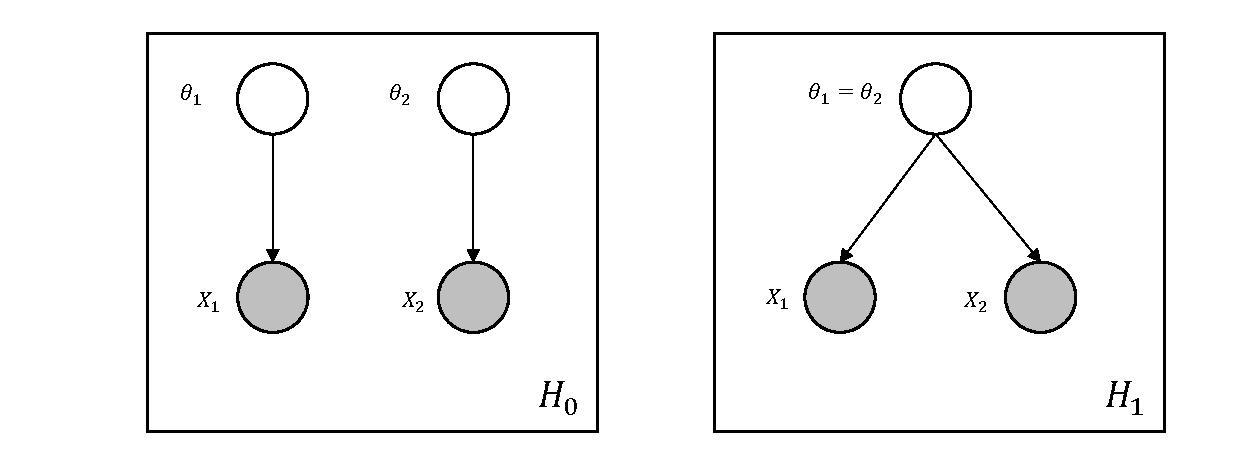
\includegraphics[scale=0.7]{img/h1h2}
  \caption[Probabilistic modeling of word merging]{Graphical model of the
  hypotheses $H_0$, $H_1$. $H_0$ represents the scenario in which two words
  $X_i, X_j$ are generated by two distinct Bernoulli processes independently
  parameterized with $\theta_1$, $\theta_2$. $H_1$ explicitly demands that the
  observations are generated by a single generative process.}
  \label{fig:hypotheses}
\end{center}
\end{figure} 

The goal is now to calculate the probabilities
of the competing hypotheses $H_0, H_1$ given the observed data. This will be
done in Section \ref{ssec:bayesian-hypothesis-testing} using \emph{Bayesian
Hypothesis Testing}.
However, before being able to apply methods of Bayesian Hypothesis Testing, we
need to establish estimates for the parameters of the underlying 
Bernoulli processes.

\subsubsection{Maximum Likelihood Estimation}
\label{ssec:mle}
When there is no further knowledge about the generative process, a commonly used
method to estimate the parameters of an assumed underlying distribution 
is the Maximum Likelihood Estimation (MLE) \cite{casellar}, i.e. parameters are
chosen such that the likelihood of the assumed underlying generative process
is maximized given the available, observed data. As shown in
\cite{myung2003tutorial}, in case of a Bernoulli process $n$ trials and $k$
successes the MLE is

\begin{equation*}
\hat{\theta}_{\mli{MLE}} = \arg \max\limits_{\theta'} B(n,k,\theta') =
\frac{k}{n}
\end{equation*}

Let $k_i, k_j$ bet the occurrences of $v_i, v_j$ in the positive class.
For the hypothesis $H_0$ postulated in the previous section, the MLEs for
each Bernoulli process generating $X_i$, are the following:

\begin{equation*}
	H_0: \hat{\theta}_{H_0,i} = \frac{k_i}{n_i}
\end{equation*}

For the second hypothesis, we assume that the independent observations $X_i, X_j$
have the same underlying distribution parameter. Assuming this hypothesis is
true, the MLE for $H_1$ is

\begin{equation*}
H_1: \hat{\theta}_{H_1} =\hat{\theta}_{H_1,1} =
\hat{\theta}_{H_1,2} =
\frac{k_i + k_j}{n_i + n_j}
\end{equation*}

Using these estimates, in the next section we describe how to use \emph{Bayesian
Hypothesis Testing} to asses the probability of either hypothesis.

\subsection{Bayesian Hypothesis Testing}
\label{ssec:bayesian-hypothesis-testing}

\emph{Bayesian Hypothesis Testing} is a tool to estimate the probability of
competing models. In our context, we want
to compare how well the occurrences of two words $v_i, v_j$ in a document set $D$ is
explained before and after merging them, either decision being represented by
the hypotheses $H_0$ and $H_1$ respectively. 
We start from the proposition, that either $H_0$ or $H_1$ are true, i.e.

\begin{equation}
	\label{eq:bayes-one}
	\Pr(H_0 \lor H_1 \given D) = \Pr(H_0 \given D) + \Pr(H_1 \given D) = 1
\end{equation}

The probabilities of the hypotheses $H_i,~i=0,1$, i.e. the
words are generated by two different Bernoulli processes or by the same one, can be expressed using the
Bayesian Rule (see Section \ref{sssec:mnb}) as follows:

\begin{equation*}
\begin{split}
\Pr(H_0\given D) &= \frac{\Pr(D \given H_0)\Pr(H_0)}{\Pr(H_0)\Pr(D \given  H_0) + \Pr(H_1)\Pr(D \given H_1)} \\
\Pr(H_1 \given D) &\stackrel{(\ref{eq:bayes-one})}{=} 1-\Pr(H_0 \given D) 
\end{split}
\end{equation*}

In Bayesian terminology, the probabilities $P(D \given H_i), i=1,2$ are also called model likelihoods
and are given by assuming an underlying distribution, in our case the Bernoulli process (see also Section \ref{sssec:mnb}). 
Note that since the hypotheses $H_0, H_1$ are complementary, computing the probability of either one 
of them yields the probability of the other one if it is subtracted from 1.
Without loss of generality, in the following we will only use $\Pr(H_0 \given D)$ since it also fulfills
the requirement for a dissimilarity measure, i.e. higher probabilities mean higher distributional 
incompatibility. For the sake of brevity, we first simplify $\Pr(H_0 \given D)$ as follows:

\begin{equation*}
\begin{split}
	\Pr(H_0|D) &= \frac{\Pr(D \given H_0)\Pr(H_0)}{\Pr(H_0)\Pr(D \given H_0) + \Pr(H_1)\Pr(D \given H_1)} \\
			 & =\frac{1}{1+
			 \underbrace{\frac{\Pr(H_1)}{\Pr(H_0)}\frac{\Pr(D \given H_1)}{\Pr(D \given H_0)}}_{
			 \eqqcolon \kappa}} \\
			 &= (1+\kappa)^{-1} \\
\end{split}
\end{equation*}

Note that since $\Pr(H_0 \given D)$ depends only the term $\kappa$, 
we will proceed by first deriving an estimate for $\kappa$ and then inserting it back in the estimate for $\Pr(H_0 \given D)$ 
at the end of our argumentation \footnote{Here $\kappa$ is called the \emph{Bayes Factor} and is often used as an
alternative to the probability to express the plausibility of $H_0$ over $H_1$.}.
Moreover, from now on we will refer to $\Pr(H_0 \given D)$ as \emph{semantic-distributional dissimilarity} 
or \emph{semantic-distributional distance}.

\subsection{Estimation of the semantic-distributional distance measure}

In this section, we derive an estimate for each probability of the Bayesian model. 
The probability estimates of the corresponding estimated probabilities will be denoted as follows:

\begin{equation}
\begin{split}
\hat{P}(H_0 \given D) &\coloneqq \left(1 + \hat{\kappa}\right)^{-1} \\
\hat{\kappa} &\coloneqq \frac{\hat{P}(H_0)\hat{P}(D \given H_0)}{\hat{P}(H_1)\hat{P}(D \given H_1)} \\
\end{split}
\end{equation}  

The following considerations are based on a pair of words $v_i, v_j \in V=\mli{voc}(D)$, where $D$ is labeled 
dataset. $X_i, X_j$ are the corresponding random variables that model the occurrences of $v_i$ as a generative process. 
Moreover, with $k_i, n_i, k_j, n_j$ are used to denote the word frequencies in the positive class and in the whole 
dataset of $v_i, v_j$ respectively, i.e

\begin{equation*}
\begin{split}
	k_i &= N_{v_i,+}^D,~n_i = N_{v_i}^D \\
	k_j &= N_{v_j,+}^D,~n_j = N_{v_j}^D	 
\end{split}
\end{equation*}   

\subsubsection{Estimation of model likelihoods}

We proceed by using the framework of \emph{Bayesian Hypothesis Testing} to derive estimates 
for the probability $\Pr(H_0 \given D)$. For this purpose, we estimate the likelihoods $\Pr(D \given H_i), i=0,1$ 
by making the following assumptions 
\begin{enumerate}
  \item Word occurrences are modeled by a Bernoulli distribution with the probability density function $B(n,k, \theta)$  (see Section \ref{sec:bernoulli}) 
  \item For word co-occurrences we assume conditional independence (c. i.) (see Section \ref{sssec:mnb})   
\end{enumerate}

Moreover, we parmeterize the assumed Bernoulli distribution with the MLEs described in Section \ref{ssec:mle} and for $\Pr(D \given H_0)$ 
we obtain the following estimate:

\begin{equation}
\begin{split}
\hat{P}(D \given H_0) &= \hat{P}\left(X_i=k_i, X_j=k_j \mid \theta_1 = \hat{\theta}_{H_0,1}, \theta_2 = \hat{\theta}_{H_0,2}\right) \\
				      &\stackrel{\text{c.i.}}{=} B(n_i,k_i,\theta_{H_0,1}) \cdot B(n_j,k_j,\theta_{H_0,2}) \\
					  &= \binom{n_i}{k_i}\hat{\theta}_{H_0,1}^{k_i}\left(1-\hat{\theta}_{H_0,1}\right)^{n_i-k_i}\cdot\binom{n_j}{k_j}\hat{\theta}_{H_0,2}^{k_j}\left(1-\hat{\theta}_{H_0,2}\right)^{n_j-k_j}
\end{split}
\end{equation}

Analogously, for $\Pr(D \given H_1)$ the estimate is 

\begin{equation}
\begin{split}
\hat{P}(D \given H_1) &= \hat{P}\left(X_i=k_i, X_j=k_j \mid \theta_1 = \theta_2 = \hat{\theta}_{H_1}\right) \\
					  &\stackrel{c.i.}{=} B(n_i,k_i,\theta_{H_1}) \cdot B(n_j,k_j,\theta_{H_1}) \\
					  &= \binom{n_i}{k_i}\binom{n_j}{k_j}\hat{\theta}_{H_1}^{k_i + k_j}\left(1-\hat{\theta}_{H_1}\right)^{n_i + n_j - k_i - k_j}
\end{split}
\end{equation}

We then insert $\hat{P}(D|H_i),~i=0,1$ in the the estimate $\hat{\kappa}$ for $\kappa$

\begin{equation}
\label{eq:bayes-factor}
\hat{\kappa} = \frac{\hat{P}(H_0)}{\hat{P}(H_1)} \cdot
\frac{\hat{\theta}_{H_0,1}^{k_i}\left(1-\hat{\theta}_{H_0,1}\right)^{n_i-k_i}\hat{\theta}_{H_0,2}^{k_j}\left(1-\hat{\theta}_{H_0,2}\right)^{n_j-k_j}
}{\hat{\theta}_{H_1}^{k_i + k_j}\left(1-\hat{\theta}_{H_1}\right)^{n_i +
n_j - k_i - k_j}}
\end{equation}

\subsubsection{Integration of semantic knowledge in the priors}
The only probabilities left for estimation are the priors $\Pr(H_0), \Pr(H_1)$.
In Bayesian models, the prior probabilities are often used as an interface for
incorporating prior, expert knowledge in the underlying models. When there is
no further knowledge about the prior probabilities $\Pr(H_0), \Pr(H_1)$ a common
heuristic is to assume that every hypothesis is equally probable, i.e. $\hat{P}(H_0) = \hat{P}(H_1) = 0.5$
\cite{zacks1971theory}. However, we can use the information provided by word 
embeddings to approximate the priors. The calculation of word
vectors implies predicting the probability of a word appearing in a given
context. The cosine similarity between two word vectors, can be interpreted as
an approximation of the probability that two words $v_i, v_j$ in question appear
in the same context $C$ \cite{mikolov2013distributed, mikolov2013efficient} (see also Section \ref{sec:skip-gram-model}). 

\begin{equation*}
	1 - \cos \angle (vec(v_i), vec(v_j)) \propto 1-\Pr(\text{``}v_i,
	v_j~\text{appear in similar contexts} \text{``})
\end{equation*}

We can use this interpretation of the cosine similarity to incorporate the
knowledge captured by word embeddings in the priors in combination with 
a regularization parameter $\alpha \in [0,1]$: 

\begin{equation}
\label{eq:priors-alpha}
\begin{split}
	\hat{P}(H_0; \alpha) &\coloneqq \alpha\cdot\left(\frac 1 2 -
	dist_\mathcal{W}(v_i,v_j)\right) + \frac 1 2
	\\
	\hat{P}(H_1; \alpha) &\coloneqq 1 - \hat{P}(H_0; \alpha)
\end{split}
\end{equation}

For words that are farther away in the embedding vector space, we want to
favor the first hypothesis, i.e. the words should not be merged. When
words are closer they tend to appear in similar contexts, which could be a hint
that the two words can be merged without losing discriminative information. 
However, as demonstrated in previous examples (see Section \ref{sec:naive-approach}), 
depending on the classification task, similarity in the word vector space is not always a good indicator for
beneficial substitutions. We therefore introduce a parameter $\alpha \in [0,1]$, that
regularizes how much the cosine distance affects the priors to deviate from 
$0.5$. For $\alpha=0$ the cosine similarity is completely neglected and the hypotheses are assumed to be equally probable. 
For $\alpha > 0$, the priors deviate from $0.5$ proportionally to $\alpha \cdot
\mli{dist}(v_i,v_j)$.\footnote{As a reminder:
$\mli{dist}_\mathcal{W}(v_i,v_j)$ is the $[0, 1]$-normalized cosine distance
between word vectors as introduced in Section \ref{sec:skip-gram-model}}

After inserting the priors above in $\hat{\kappa}$ , we obtain this result 

\begin{equation}
\label{eq:bayes-factor-alpha}
\begin{split}
	\hat{\kappa} &= \kappa(\alpha) = \frac{\hat{P}(H_0; \alpha)}{1-\hat{P}(H_0; \alpha)}\frac{\hat{P}(D|H_1)}{\hat{P}(D \given H_0)} \\		
		   &= \frac{\alpha\cdot\left(\frac 1 2 - dist_\mathcal{W}(v_i,v_j)\right) + \frac 1 2}{\frac 1 2 - \alpha\cdot\left(\frac 1 2 - dist_\mathcal{W}(v_i,v_j)\right)} \cdot \frac{\hat{\theta}_{H_0,1}^{k_i}\left(1-\hat{\theta}_{H_0,1}\right)^{n_i-k_i}\hat{\theta}_{H_0,2}^{k_j}\left(1-\hat{\theta}_{H_0,2}\right)^{n_j-k_j}}{\hat{\theta}_{H_1}^{k_i + k_j}\left(1-\hat{\theta}_{H_1}\right)^{n_i + n_j - k_i - k_j}} 
\end{split}
\end{equation}

Finally, we define the \emph{semantic-distributional distance}, that incorporates both distributional and semantic information about 
the measured words, as follows:

\begin{equation}
	\label{eq:dist-v1v2}
	\Lambda_{\alpha, \mathcal{W}}(v_i, v_j) \coloneqq \hat{P}(H_0 \given D)= \left(1 +
	\hat{\kappa}(\alpha) \right)^{-1}
\end{equation}

We note that that $\Lambda_{\alpha, \mathcal{W}}(v_i, v_j)$ was defined using the cosine distance of word vectors in an 
embedding $\mathcal{W}=(V_{\mathcal{W}}, (\mathbf{x}_i)_i)$. Therefore, in order to produce valid distances, 
it requires $v_i, v_j$ to be part of the vocabulary $V_\mathcal{W}$.


\subsection{Adding a linear correction term}
\label{ssec:adding-linear-correction-term}
Upon inspecting the clustering quality using the semantic-distributional distance measure 
introduced in previous sections, we noticed that the distributional portion of information, 
given by the likelihoods $\hat{P}(D\given H_i), i=1,2$, dominated over the semantic information. As a consequence, 
the resulting clusters partially lost semantic coherence. 
We suppose that this effect is due the assumption of a \emph{linear} relationship between the priors $\hat{P(H_i)}$ 
and the cosine distance $dist_\mathcal{W}$ (see Equation \ref{eq:priors-alpha}). Moreover, we  
conjecture that this assumption undervalues the semantic similarity between the measured words. 
 For this purpose we add a correction term regularized by a parameter $\beta \in [0,1]$ as follows:   

\begin{equation*}
	\Lambda_{\alpha,\beta, \mathcal{W}}(v, v') = \beta \Lambda_{\alpha,\mathcal{W}}(v,v')
	+ (1-\beta)\mli{dist}_\mathcal{W}(v,v'), \beta \in [0,1]
\end{equation*}

The parameter $\beta \in [0,1]$ regulates the extent to which the word similarity $\mli{dist}_\mathcal{W}$ 
is added as a correction term to the semantic-distributional distance measure. 
Even though this approach is rather engineered than theoretically motivated, the results of our experiments 
seem to indicate that the combination of distributional and semantic information is beneficial to TC tasks.
As matter of fact, our method we achieves improvements in classification accuracy in all the datasets evaluated.
Possible future work could consist of finding a probabilistically motivated approach to include 
semantic information in the priors, without the need of a correction term.   

 \subsection{Relationship to the weighted Jensen-Shannon Divergence}

In \cite{baker1998distributional} Baker et al. propose a weighted variant of the
Jensen-Shannon divergence to calculate the information loss when merging two
words:

\begin{equation*}
\begin{split}
D_{WJS}(v_1, v_2) \coloneqq &\Pr(v_1) \cdot
\mathbb{D}\left(\Pr(\omega|v_1)\Vert\Pr(\omega \given  v_1 \lor v_2)\right) + \\  
&\Pr(v_2) \cdot \mathbb{D}\left(\Pr(\omega \given v_2)\Vert\Pr(\omega\given v_1
\lor v_2)\right)
\end{split}
\end{equation*} 

Here $\mathbb{D}(\cdot \Vert \cdot)$ indicates the Kullback-Leibler divergence,
which is used to measure the difference between distributions.
In \cite{baker1998distributional} the Jensen-Shannon divergence is used to 
quantify the difference of the distributions of a (1) word being viewed as a
single probabilistic event and the (2) collapsed event after merging two words. 
For $\Pr(H_0) = \Pr(H_1) = 0.5$, we found empirical evidence that $\Pr(H_1\given
D)$ correlates exponentially with their metric (see Figure \ref{fig:jensen-shannon}).

%\usepackage{graphics} is needed for \includegraphics
\begin{figure}[htp]
\begin{center}
  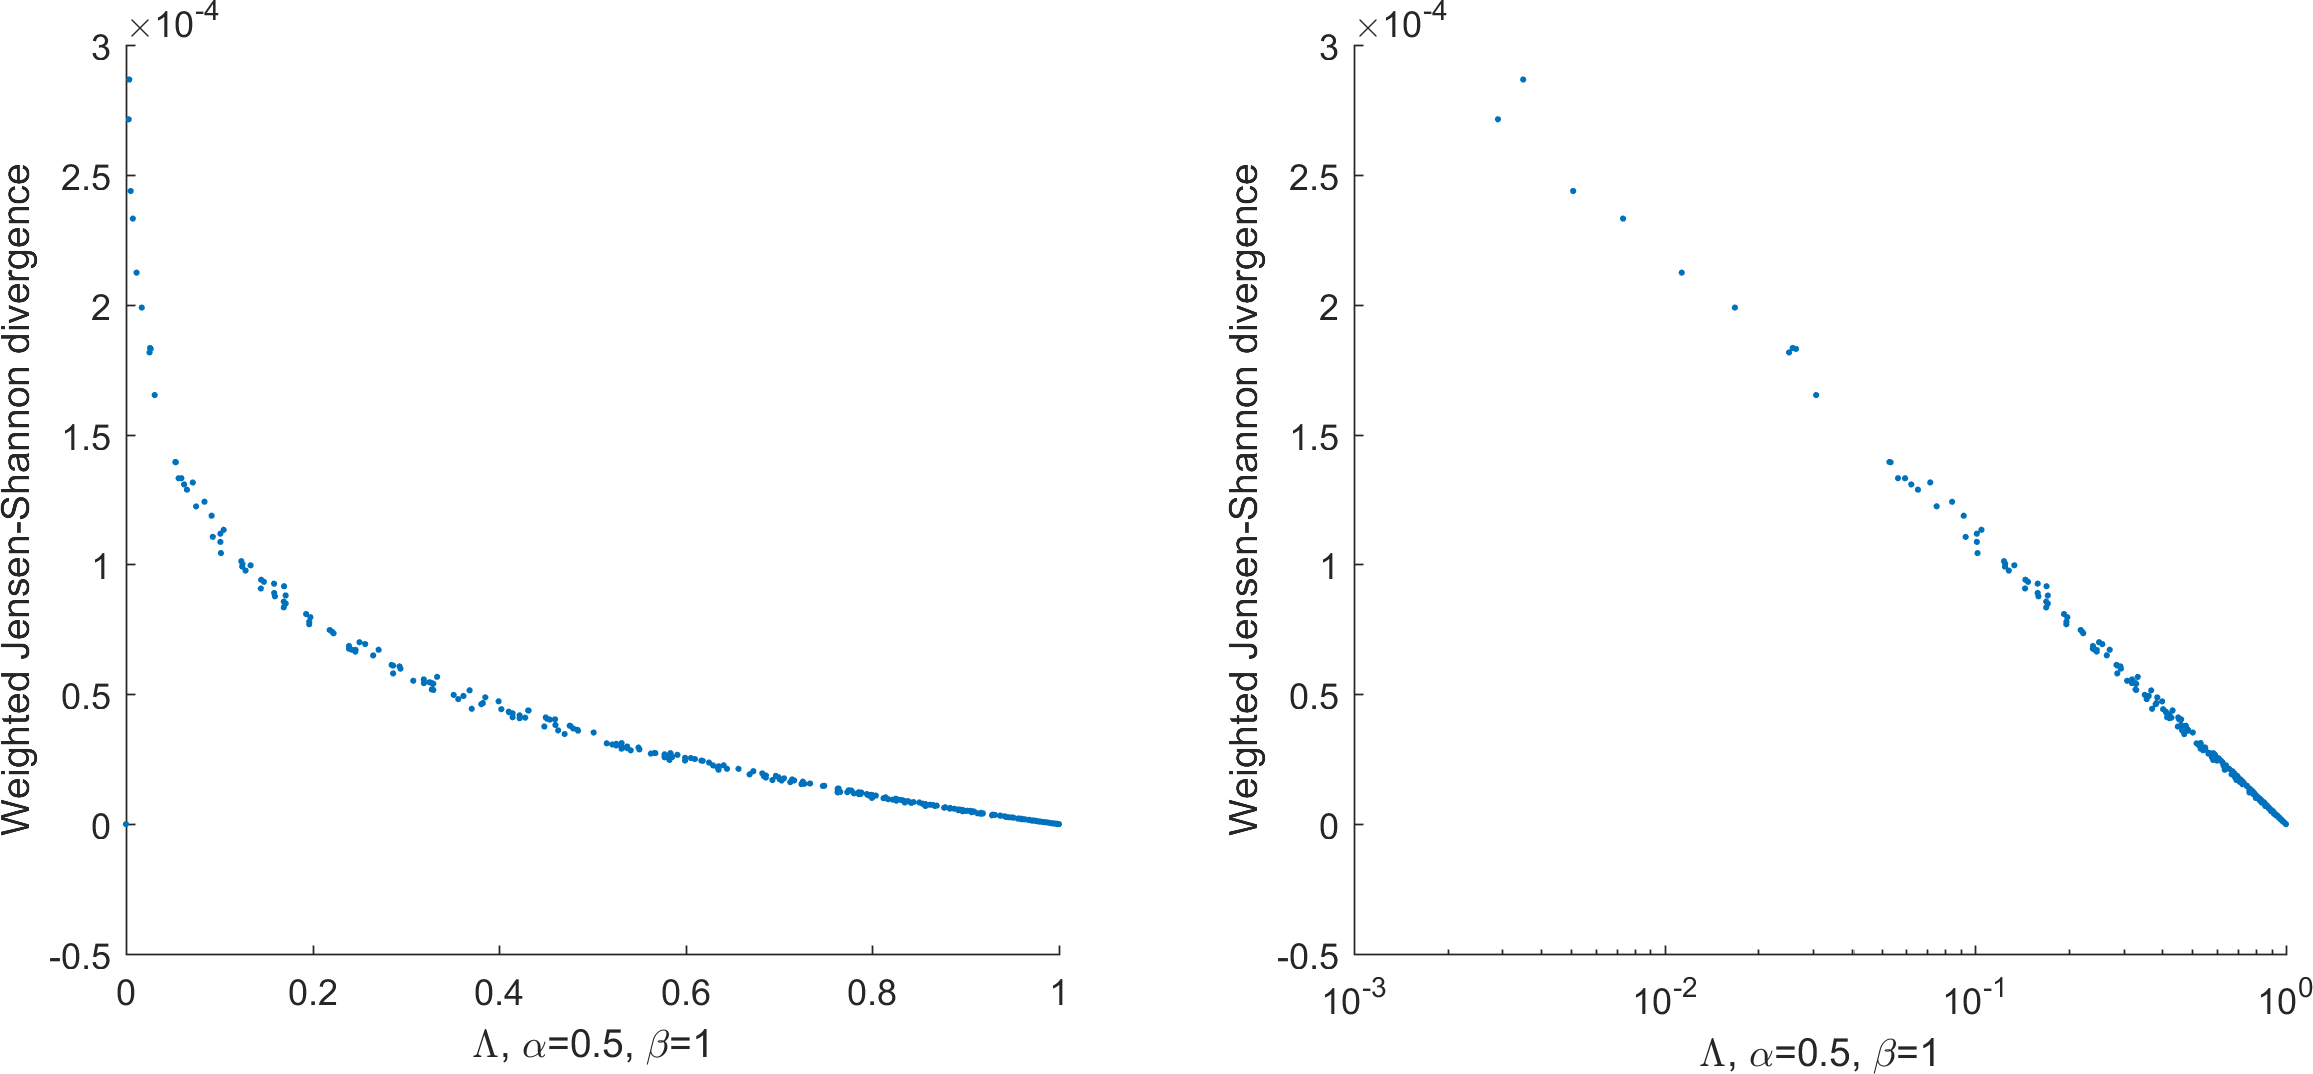
\includegraphics[scale=0.5]{img/correlation-metric}
  \caption[Correlation of $\Lambda_{\alpha, \beta,\mathcal{W}}$
  with $\alpha=0, \beta=1$ with weighted Jensen-Shannon distance]{We
  computed the distributional distance proposed in
  \cite{baker1998distributional} and plotted it over the distance measure
  proposed in this work with $\alpha = 0, \beta=1$. The left and the right plot
  represent the X-Axis in a linear and logarithmic scale respectively.
  Upon visual inspection, we conclude that there must be an exponential
  relationship between $\Lambda_{\alpha, \beta,\mathcal{W}}$ with $\alpha=0, \beta=1$ and the weighted Jensen-Shannon distance.}
  \label{fig:jensen-shannon}
\end{center}
\end{figure}

However, the main advantage of using our method, is the possibility to
incorporate prior knowledge in $\Pr(H_i), i=0,1$, which is naturally offered 
by modeling the problem under the Bayesian theorem. Moreover, as opposed to 
the results reported in \cite{baker1998distributional}, with our method we 
achieve improvements in all the evaluated datasets.

\section{Implementation of the Preprocessing Procedure}

Up until now we considered the pairwise distance between words $v, v' \in V$. As
mentioned in Section \ref{sec:lex-sub-boc}, the goal is to find \emph{clusters}
of similar words and use them for lexical substitution. In the following
sections we provide a method for preprocessing datasets using the 
distance measure derived in this work. We propose to use a greedy
agglomerative clustering algorithm (Section \ref{ssec:clustering}) to find groups of
similar words inn order to perform lexical substitution as described
in Section \ref{sec:lex-sub-boc}. In Section \ref{ssec:n-grams-distance}, we 
introduce a distance measure based on $N$-Grams, which ultimately will allow to use 
them in the lexical substitution process. 
Finally, we demonstrate how to automatically map OOV-words contained in unknown documents to words known by
the classification model (Section \ref{ssec:oov-automated}). 
In section \ref{ssec:preprocessing-algorithms} we provide the Pseudo-Code of the algorithms
for preprocessing the datasets evaluated in Chapter \ref{ch:Evaluation}. 


\subsection{Greedy Agglomarative Hierarchical Clustering}
\label{ssec:clustering}

Let $V = \{v_1,\ldots,v_{|V|}\}$ be a set of terms of a document set $D$ and
$\mathbf{W}=(w_{ij}) \in \mathbb{R}^{|V|\times|V|}$ a symmetrical \emph{dissimilarity matrix}, 
where the elements $w_{ij}$ indicate dissimilarity between the term $v_i$ and
$v_j$ according to our distance function $\Lambda_{\alpha, \beta, \mathcal{W}}$,
i.e.
$w_{ij} = \Lambda_{\alpha, \beta, \mathcal{W}}(v_i, v_j) = \Lambda_{\alpha,
\beta, \mathcal{W}}(v_j, v_i) = w_{ji}$.

\emph{Greedy Agglomerative Hierarchical Clustering} is a bottom-up
clustering algorithm, i.e. it starts from the premise that at first (step
$i=0$) every word $v \in V$ is a cluster. At each step $i$ the clusters are merged pairwise into bigger
clusters. The algorithm stops, when there are $K$ clusters left. The criterion
to decide whether to merge two clusters or not is based on the dissimilarity
matrix $\mathbf{W} = (w_{ij})$ and a \emph{linkage criterion} $\lambda$. At
step $i>0$ a cluster $C$ is merged with the closest cluster $C' \neq C$, i.e.

\begin{equation*}
 C' = \min\limits_{C'' \in \mathcal{C}_{i-1}} \lambda(C,C'') 
\end{equation*}

where $\mathcal{C}_{i-1}$ denotes the clustering yielded at step $i-1$.
Possible functions that can be chosen for $\lambda$ are e.g. the minimum, the
maximum or the average distance between words in the different clusters. 
In order to make sure that every word best fits in the assigned
cluster, we chose the \emph{maximum}, it being the most conservative linkage criterion.  

\begin{equation*}
	\lambda(C,C') = \max\limits_{v_i \in C, v_j \in C' } w_{ij} 
\end{equation*}

When the algorithm stops it outputs a clustering $\mathcal{C} = \left\{ C_1,\ldots,C_K \right\} $ 
over $V$, where $C_k \subset V, C_k \cap C_{k'} = \emptyset,~k \neq
k'$. 

Using $\lambda$ as above is also known as \emph{complete-linkage clustering}.
As opposed to \emph{single-linkage}, where two clusters are merged together
based on their \emph{closest} members, complete-linkage clustering avoids the
so called \emph{chaining phenomenon}, i.e. clusters that have many elements
that are very distant to each other might be merged because of their closest
elements.

The advantage of using agglomerative clustering, is that it allows to operate on
a dissimilarity matrix based on \emph{any} distance function designed by the
user of the algorithm. On the other hand, clustering algorithms like $K$-means
or DB-Scan require the actual observations, which in our case are not available.
 However, a property shared with $K$-means is that the number of clusters $K$ 
 has to be chosen by the user of the algorithm as a parameter (see Chapter
 \ref{ch:Evaluation}).

\subsection{Distance measurement on N-Grams}
\label{ssec:n-grams-distance}
When using $N$-Grams, it is very likely that there is no
corresponding vector representation in the embedding vector space. However, in
order to be able to measure the distance between $N$-Grams, we use the
\emph{maximal distance} between the corresponding unigrams. E.g. the distance
between the bigrams $u='(\text{``new'', ``CEO''})$ and $v=(\text{``future''},
\text{``Manager''})$ is defined as

\begin{equation*}
	\mli{dist}_2(u,v) = \max(\mli{dist}(\text{'new'}, \text{{'future'}}),
	\mli{dist}(\text{'CEO'}, \text{'Manager')})
\end{equation*}

More generally, we define the distance measure of word vectors for any size
$N=n$ of $N$-Grams $u,v \in V_n$:

\begin{equation*}
\begin{split}
	v &\coloneqq (v_1,v_2,\ldots,v_n) \in V_n \\
	u &\coloneqq (u_1,u_2,\ldots,u_n) \in V_n \\
	\mli{dist}_\mathcal{W}^{(n)}(v,v') &\coloneqq \max\limits_{i \in \left\{
	1,\ldots, n \right\}} dist_\mathcal{W}(u_i, v_i)
\end{split}
\end{equation*}

Correspondingly, we define a distance measure
$\Lambda^{(n)}_{\alpha,\beta,\mathcal{W}}$ that can be employed with $N$-Grams

\begin{equation*}
\Lambda_{\alpha,\beta,\mathcal{W}}^{(n)}(u,v) \coloneqq \beta B(u,v; \alpha) +
(1-\beta)\mli{dist}_\mathcal{W}^{(n)}(u,v)
\end{equation*}

and a dissimilarity matrix  $\mathbf{W}^{(n)}$ over $N$-Grams $V_n$ based
on $\Lambda_{\alpha,\beta,\mathcal{W}}^{(n)}$:

\begin{equation*}
\begin{split}
	\mathbf{W}^{(n)} &\in [0,1]^{|V_n|\times|V_n|} \\
	\mathbf{W}^{(n)} &\coloneqq \left(w^{(n)}_{ij}\right) \\
	w^{(n)}_{ij} &\coloneqq \Lambda_{\alpha,\beta,\mathcal{W}}^{(n)}(v_i,v_j), v_i,
	v_j \in V_n
\end{split}
\end{equation*}

\subsection{Mapping OOV-words to known Vocabulary}
\label{ssec:oov-automated}
An unknown document $\tilde{d} \in \mathcal{D}\setminus D$ might contain words not
known by the classifiers, i.e. $\tilde{v} \in \mathcal{V}\setminus V$. Prior to
classification, we substitute every word $\tilde{v} \in
\mathcal{V} \setminus V$ with the closest word $v \in V$ with respect
to $\mli{dist}_\mathcal{W}$. If the closest word is further away than $\theta_d$
we discard it. The mapping of OOV-words can be formally described as a preprocessing function $\tau$ as follows:

\begin{equation*}
\begin{split}
	\tilde{d} &= (\tilde{w}_1, \ldots, \tilde{w}_{|\tilde{d}|}) \in
	\mathcal{D}\setminus D \\	
	\boldsymbol\tau(\tilde{d}) &= (\tau(\tilde{w}_1), \ldots,
	\tau(\tilde{w}_{|\tilde{d}|})) \\	
	\tau(\tilde{w}) &= \begin{cases} \tilde{w} & \text{if~} \tilde{w} \in V \\ v' &
	\text{if~} v' = \arg\min\limits_{v''\in V}\mli{dist}(\tilde{w},v'') 
	\text{~and~} \mli{dist}(v',\tilde{w}) \leq \theta_d \\ \epsilon
	& \text{otherwise}
	\end{cases}	
\end{split} 
\end{equation*}

Here $\epsilon$ is the \emph{empty word} and simply denotes that a word is removed
from the document in case there is no suitable substitute satisfying the
constraint given by the distance threshold.

\subsection{Preprocessing Algorithms}
\label{ssec:preprocessing-algorithms}
The preprocessing of a dataset involves finding clusters using the distance
measure introduced in Section \ref{sec:distance-measure} and then represent each
document as a BoC. Subsequently a classification model with the preprocessed
training dataset is built. Prior to prediction, unknown documents that contain
OOV-words are preprocessed by substituting unknown words with vocabulary
contained in the training dataset. In the previous sections we showed how to
perform every single step. In the following sections provide details about the
whole preprocessing chain.

\subsubsection{Preprocessing Training Data}

Listing \ref{alg:preprocess-training-data} shows a qualitative algorithm of
how we intend to preprocess the training data prior to building a
classification model. 

\begin{algorithm}

\label{alg:preprocess-training-data}
\caption{Algorithm structure for preprocessing training data}
\begin{algorithmic}[1]
\Function{PreprocessTrainingData}{$\protect D$, $\protect \mathcal{W}$,
$\protect N$, $\protect \boldsymbol \alpha[1..N]$, $\protect
\boldsymbol \beta[1..N]$, $\protect \boldsymbol K[1..N]$}
\label{alg:preprocess-training-data:parameters}
\State $D_N^* \gets g_N^*(D)$ \Comment{Append $2,\ldots,N$-Grams to each
document}
\label{alg:preprocess-training-data:n-grams}
\State $V_N^* \coloneqq \mli{voc}(D_N^*)$
\State $V_N^* \gets V_1 \cup V_2 \cup \ldots \cup V_N$
\State $\mathcal{C} \coloneqq \emptyset$
\For{$n \in \left\{1,\ldots,N\right\}$}
\label{alg:preprocess-training-data:loop}
\State $\mathbf{W}^{(n)} \coloneqq \mli{pairwise-distances}(V_n,
\Lambda_{\boldsymbol \alpha[n], \boldsymbol \beta[n], \mathcal{W}}^{(n)})$

\State $\mathcal{C}^{(n)} \coloneqq
\mli{complete-linkage-cluster}(\mathbf{W}^{(n)}, \boldsymbol K[n])$
\State $\mathcal{C} \gets \mathcal{C} \cup \mathcal{C}^{(n)}$
\EndFor
\State $\mathbf{F} \gets \mli{bag-of-clusters}(D_N^*, \mathcal{C})$
\label{alg:preprocess-training-data:boc} 
\Comment{The final feature matrix used for training}
\State \Return $(\mathcal{C}, V_N^*, \mathbf{F})$
\EndFunction
\end{algorithmic}
\end{algorithm}

The preprocessing step accepts a dataset $D$, the size of $N$-Grams to be used
$N$, metric parameters $\boldsymbol \alpha, \boldsymbol \beta$ and a clustering
parameter $\boldsymbol K$ (Line \ref{alg:preprocess-training-data:parameters}).
Each $N$-Gram level is parameterized with its own parameter set, i.e. for
$N$-grams of size $N=n$ we use parameters $\boldsymbol\alpha[n],
\boldsymbol\beta[n]$ and $\boldsymbol K[n]$ for the distance metric $\Lambda_n$
and the clustering algorithm respectively. In Line
\ref{alg:preprocess-training-data:n-grams} the document is affixed with
$N$-Grams of size $1,\ldots,N$. In the loop on line
\ref{alg:preprocess-training-data:loop} we iterate over the different
sizes of $N$-grams ($n=1,\ldots,n$) and calculate the respective dissimilarity
matrix based on $\Lambda_n$ and the a complete-linkage clustering with $\boldsymbol K[n]$ clusters. 
All clustering are accumulated in $\mathcal{C}$ and finally used to represent
the document as a bag-of-clusters (Line \ref{alg:preprocess-training-data:boc}). The matrix
$\mathbf{F}$ is the resulting feature matrix of the type
$\mathbb{N}^{|D|\times|\mathcal{C}|}$ (number documents $\times$ number of clusters) that is later used for training a
classifier. Each row of the matrix represents a document and each column the
number of occurrences of the members of the corresponding cluster in
$\mathcal{C}$.

Using a different parameter set for each $N$-gram level allows adapt the
parameters in order to account for the different distributional properties of
higher order $N$-grams: With $N$ growing the features become more sparse and a
heavier feature reduction (smaller $K$) might be needed to compensate low
feature counts.
$\boldsymbol \alpha, \boldsymbol \beta$ regulate how much the semantic information is weighed against the distributional information in
the distance measurement function. For higher $N$-grams it might be necessary to
increase the weights in favor of semantic information, since the counts become 
lower and thus less reliable for probability estimation. 

\subsubsection{Preprocessing unknown Documents}

After having built a classification model using the preprocessed training data,
we want to use it to predict classes of unknown documents. Prior to prediction,
unknown documents have to mapped to feature vectors $\mathbf{\tilde{f}} \in
\mathbb{N}^{|\mathcal{C}|}$. Also, since they might contain words not known by
the classifier, a mapping procedure to known vocabulary has to be performed. Listing
\ref{alg:preprocess-unknown-data} illustrates a possible algorithm for
preprocessing unknown documents as described.

\begin{algorithm}
\label{alg:preprocess-unknown-data}
\caption{Preprocessing of unknown documents}

\begin{algorithmic}[1]
\Function{PreprocessUnknownDocuments}{$\protect \tilde{D}$, $N$, $V_N^*$,
$\boldsymbol\theta_d[1..N]$, $\mathcal{C}$}

\State $\tilde{D}_N^* \coloneqq g_N^*(\tilde{D})$ 
\label{alg:preprocess-unknown-data:n-grams}
\State $\tilde{V}_N^* \coloneqq \mli{voc}(\tilde{D}_N^*)$

\State $V_N^* \gets V_1 \cup V_2 \cup \ldots \cup V_N$ 
\label{alg:preprocess-unknown-data:n-grams-known-partition}
\State $\tilde{V}_N^* \gets \tilde{V}_1 \cup \tilde{V}_2 \cup \ldots \cup
\tilde{V}_N$
\label{alg:preprocess-unknown-data:n-grams-unknown-partition}

\For{$n \in \{1,\ldots,N\}$}
\State $\tilde{V} \coloneqq \tilde{V}_n \setminus V_n$
\State $\mli{NN} \coloneqq \mli{nearest-neighbor}(\tilde{V}, V_n,\mathcal{W},
\mli{dist}_n) \subset \tilde{V} \times V_n \times ([0,1]\cup\{\infty\})$ 
\label{alg:preprocess-unknown-data:nearest-neighbor}
\State $S \coloneqq \left\{(\tilde{v}, v) \mid (\tilde{v}, v,d) \in \mli{NN}
\land d \leq \boldsymbol \theta_d[n]\right\}$
\label{alg:preprocess-unknown-data:substitutes} 
\State $R \coloneqq \left\{\tilde{v} \mid (\tilde{v}, v,d) \in \mli{NN}
\land d > \boldsymbol \theta_d[n]\right\}$ 
\State $\tilde{D}_N^* \gets \mli{substitute}(\tilde{D}_N^*,S)$
\State $\tilde{D}_N^* \gets \mli{remove}(\tilde{D}_N^*,R)$
\label{alg:preprocess-unknown-data:substitutes-end}
\EndFor

\State $\mathbf{\tilde{F}} \coloneqq \mli{bag-of-clusters}(\tilde{D}_N^*, 
\mathcal{C})$ 
\label{alg:preprocess-unknown-data:boc}
\State \Return $\mathbf{\tilde{F}}$
\EndFunction
\end{algorithmic}
\end{algorithm}

The algorithms input is a set of unknown documents $\tilde{D}$, the $N$-gram
size $N$, distance thresholds $\boldsymbol \theta_d[1..N]$ and a clustering
$\mathcal{C}$.

We first transform the set of unknown documents to its $N$-grams representation
(Line \ref{alg:preprocess-unknown-data:n-grams}). In lines
\ref{alg:preprocess-unknown-data:n-grams-known-partition} and 
\ref{alg:preprocess-unknown-data:n-grams-unknown-partition} we partition the known
vocabulary and the vocabulary of unknown documents into separate sizes of $N$-Grams.
 We then iterate through the
sizes of $N$-Grams and calculate the nearest neighbors of the OOV-words
$\tilde{V}$ of the corresponding $N$-Grams of size $N=n$. In line
\ref{alg:preprocess-unknown-data:nearest-neighbor}, based on the word embeddings
$\mathcal{W}$ and the distance measure $\mli{dist}_n$, the function $\mli{nearest-neighbor}$ returns triples 
of the form (OOV word $\tilde{v}$, nearest known word $v$, cosine distance
between $v$ and $\tilde{v}$). 
From this set we filter out the substitutions $S$ that satisfy the
threshold $\boldsymbol \theta_d[n]$ and the ones who do not $R$. The
string functions $\mli{substitute}$ and $\mli{remove}$ are used to substitute or
remove the words from the document set respectively (see lines
\ref{alg:preprocess-unknown-data:substitutes} --
\ref{alg:preprocess-unknown-data:substitutes-end}). In line
\ref{alg:preprocess-unknown-data:boc} the bag-of-clusters
representation of the preprocessed unknown document set is computed and returned
as feature matrix $\mathbf{\tilde{F}}$.

\subsubsection{Training and Prediction}

After defining how to preprocess raw textual data with the method proposed in
this work, we show how the preprocessed data can be incorporated in a 
classification process (see Listing \ref{alg:classification}).

\begin{algorithm}
\label{alg:classification}
\caption{Build classification model and predict class of unknown documents}

\begin{algorithmic}[1]
\Function{BuildModelAndPredict}{$D$, $L$,
$N$, $\protect \boldsymbol \alpha[1..N]$, $\protect
\boldsymbol \beta[1..N]$, $\protect \boldsymbol K[1..N]$,
$\boldsymbol\theta_d[1..N]$}

\State $(\mathcal{C}, V_N^*, \mathbf{F}) \coloneqq
\textproc{PreprocessTrainingData}(D,L,N,\boldsymbol \alpha, \boldsymbol \beta, \boldsymbol K)$ \State $M = \mli{build-classification-model}(\mathbf{F},L)$
\While{Fetch unknown documents $\tilde{D}$}
\State $\mathbf{\tilde{F}} = \textproc{PreprocessUnknownDocuments}(\tilde{D}, N,
V_N^*, \boldsymbol\theta_d, \mathcal{C})$
\State $p = M.\mli{predict}(\mathbf{\tilde{F}})$
\EndWhile

\EndFunction
\end{algorithmic}
\end{algorithm}

The feature matrix returned by \textproc{PreprocessTrainingData} is used for
building a classification model $M$. As a data source continuously provides
batches of unknown documents, they are preprocessed by reusing the clustering
computed in while preprocessing the training data.
